\documentclass[12pt]{article}

\setlength{\parindent}{0em}
\setlength{\parskip}{.5em}

\usepackage{framed}
\newcounter{problem}
\newcounter{problempart}[problem]
\newcounter{solutionpart}[problem]
\newenvironment{problem}{\stepcounter{problem}\noindent{\bf\arabic{problem}.}}{\setcounter{problempart}{0}\setcounter{solutionpart}{0}}
\newenvironment{solution}{\par\textcolor{blue}\bgroup}{\egroup\par}
\newcommand{\qpart}{\stepcounter{problempart}${}$\\\noindent{(\alph{problempart})} }
\newcommand{\spart}{\stepcounter{solutionpart}${}$\\\noindent{(\alph{solutionpart})} }
\newcommand{\TODO}{\textcolor{red}{$\blacksquare$}}
\newcommand{\SOL}[1]{\textcolor{blue}{#1}}

\usepackage{hyperref}
\usepackage{fullpage}
\usepackage{amsmath,mathabx,MnSymbol}
\usepackage{color,tikz}
\usepackage{footnote,enumitem}
\usepackage{longtable}
\newcommand{\mx}[1]{\begin{pmatrix}#1\end{pmatrix}}
\definecolor{dkgreen}{rgb}{0,.5,0}
\usepackage{algorithm}
\usepackage[noend]{algpseudocode}

\newcommand{\uu}{\mathbf{u}}
\newcommand{\vv}{\mathbf{v}}
\newcommand{\cc}{\mathbf{c}}
\newcommand{\ww}{\mathbf{w}}
\newcommand{\xx}{\mathbf{x}}
\newcommand{\zz}{\mathbf{z}}
\newcommand{\ee}{\mathbf{e}}
\newcommand{\pp}{\mathbf{p}}
\newcommand{\qq}{\mathbf{q}}
\renewcommand{\AA}{\mathbf{A}}
\newcommand{\BB}{\mathbf{B}}
\newcommand{\CC}{\mathbf{C}}
\newcommand{\DD}{\mathbf{D}}
\newcommand{\nn}{\mathbf{n}}
\renewcommand{\tt}{\mathbf{t}}
\newcommand{\gp}[1]{\left(#1\right)}

\newcommand{\TODOL}[1]{\textcolor{red}{\underline{\hspace{#1 cm}}}}

\usepackage{listings}

\lstset{
  language=C++,
  showstringspaces=false,
  identifierstyle=\color{magenta},
  basicstyle=\color{magenta},
  keywordstyle=\color{blue},
  identifierstyle=\color{black},
  commentstyle=\color{green},
  stringstyle=\color{red}
}

\begin{document}

\title{CS130 - Reflections and transparency}
\date{}
\author{Name: \TODOL7\qquad\qquad SID: \TODOL4}
\maketitle
\begin{center}
\end{center}

\begin{problem}
  Given the vector $\uu=\langle 1,4\rangle$ and the unit vector $\nn=\langle-\frac{3}{5},\frac{4}{5}\rangle$, decompose $\uu$
  into component $\uu_\perp$ perpendicular to $\nn$ and component $\uu_{\|}$
  parallel to $\nn$ such that $\uu = \uu_\perp + \uu_{\|}$.
\end{problem}

\begin{solution}
  \textbf{\textcolor{red}{\TODO}}
\end{solution}

\begin{center}
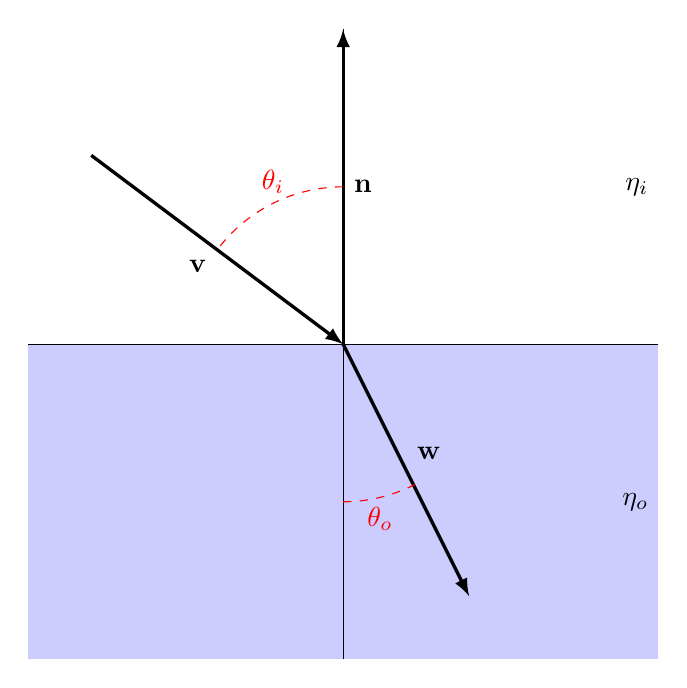
\begin{tikzpicture}[scale=1]
\draw[fill=blue!20,draw=none] (-4,-4) -- (4,-4) -- (4,0) -- (-4,0) -- cycle;
\draw[] (-4,0)--(4,0);
\draw[] (0,-4)--(0,4);
\draw[very thick,latex-] (0,0) -- node[below left]{$\vv$} (-3.2,2.4);
\draw[very thick,-latex] (0,0) -- node[above right]{$\ww$} (1.6,-3.2);
\draw[very thick,-latex] (0,0) -- node[right]{$\nn$} (0,4);
\node[left] at (4,2) {$\eta_i$};
\node[left] at (4,-2) {$\eta_o$};
\draw[dashed,red] (0,2) arc (90:143:2) node[pos=.5,above] {$\theta_i$};
\draw[dashed,red] (0,-2) arc (270:297:2) node[pos=.5,below] {$\theta_o$};
\end{tikzpicture}
\end{center}

In the figure above, a ray originally in the air (index of refraction $\eta_i$)
enters a transparent material (index of refraction $\eta_o$).  The ray enters
along direction $\vv$ and leaves along direction $\ww$.  You are given that
$\|\vv\| = 1$ and $\|\nn\| = 1$.  You will construct $\ww$ such that $\|\ww\| =
1$.  $\ww$ lies in the same plane as $\nn$ and $\vv$.

\begin{problem}
Snell's law states that $\eta_i \sin \theta_i = \eta_o \sin \theta_o$.  Express this equation in terms of the vectors $\vv$, $\nn$, and $\ww$ using cross products (no dot products).
\end{problem}

\begin{solution}
  \textbf{\textcolor{red}{\TODO}}
\end{solution}

\begin{problem}
  Taking advantage of the fact that $\ww$, $\nn$, and $\vv$ lie in the same plane, we can write $\ww = a \vv + b \nn$.  Using your result from the previous problem, solve for $a$.  Note that you will only be able to solve for $a$ up to a sign.
\end{problem}

\begin{solution}
  \textbf{\textcolor{red}{\TODO}}
\end{solution}

\begin{problem}
Let $\tt$ be a vector orthogonal to $\nn$ as shown in the figure.  Taking the dot product of $\ww = a \vv + b \nn$ by $\tt$, deduce the sign of $a$.
\end{problem}

\begin{solution}
  \textbf{\textcolor{red}{\TODO}}
\end{solution}

\begin{problem}
Using $\|\ww\|^2=1$ to derive a quadratic equation in $b$.  Solve this for $b$, which should give you two solutions.  We will select the solution we want later.
\end{problem}

\begin{solution}
  \textbf{\textcolor{red}{\TODO}}
\end{solution}

\begin{problem}
If $\vv = -\nn$, then we should get $\ww = \vv$ as our solution.  Use this special case to deduce the correct sign for $b$.  Using the $a$ and $b$ you derived, write out $\ww$.
\end{problem}

\begin{solution}
  \textbf{\textcolor{red}{\TODO}}
\end{solution}

\begin{problem}
Based on your formula for $\ww$, deduce the conditions under which complete internal reflection occurs.
\end{problem}

\begin{solution}
  \textbf{\textcolor{red}{\TODO}}
\end{solution}

\begin{problem}
What happens as the index of refraction of the sphere in \texttt{08.txt} is made closer to the index of refraction of the air?  Support your conclusion by showing a sequence of renders.  What happens when they are equal?
\end{problem}

\begin{solution}
  \textbf{\textcolor{red}{\TODO}}
\end{solution}

\end{document}
